% --------------------------------------
%                   STYLES
% --------------------------------------
% Odporúčané nastavenie: Times New Roman, veľkosť 12; riadkovanie 1,5; okraje vľavo 3,5 cm, vpravo 2 cm, zhora a zdola 2,5 cm,
\documentclass[12pt, a4paper, oneside]{book}
\linespread{1.5}

% characters counter
\newread\tmp

\newcommand{\quickcharcount}[1]{%
  \immediate\write18{texcount -1 -sum -merge -char #1.tex > #1-chars.sum}%
  \openin\tmp=#1-chars.sum%
  \read\tmp to \thechar%
  \closein\tmp%
}

\newcommand{\quickwordcount}[1]{%
  \immediate\write18{texcount -1 -sum -merge #1.tex > #1-words.sum}%
  \openin\tmp=#1-words.sum%
  \read\tmp to \theword%
  \closein\tmp%
}


% --------------------------------------
%                   HIDE IMAGES
% --------------------------------------
%\renewcommand{\includegraphics}[2][]{
%   \fbox{#2}% print file name in a small box
%}



% --------------------------------------
%                   PACKAGES
% --------------------------------------
\usepackage[slovak]{babel}
\usepackage{lipsum}
%\usepackage{newtxtext}
\usepackage{comment}
\usepackage[a4paper,top=2.5cm,bottom=2.5cm,left=3.5cm,right=2cm]{geometry}
\usepackage[utf8]{inputenc}
\usepackage[T1]{fontenc}    
\usepackage{graphicx}
\usepackage{url}
\usepackage{epsfig}
\usepackage{listings}
\usepackage{epstopdf}
\usepackage{algorithmic}
\usepackage{amssymb}
\usepackage{multirow}
\usepackage{booktabs}
\usepackage{color}
\usepackage{setspace}
\usepackage{tabularx}
\usepackage{textcomp}
\usepackage{caption}
\usepackage{natbib}
\usepackage{subcaption}
\usepackage[font=large]{subcaption}
\usepackage{emptypage}
\usepackage{float}
\usepackage[hidelinks,breaklinks]{hyperref}
\usepackage{minted}
\usepackage[thinlines]{easytable}
\usepackage{amsmath}
\usepackage{amsmath,scalerel}



% --------------------------------------
%                   PERSONAL INFO
% --------------------------------------
\newcommand\mftitle{Detekcia vizuálneho smogu pri cestách}
\newcommand\mfthesistype{Diplomová práca}
\newcommand\mfauthor{Bc. Ján Špirka}
\newcommand\mfadvisor{RNDr. Zuzana Černeková, PhD.}
\newcommand\mfplacedate{Bratislava, 2023}
\newcommand\mfuniversity{UNIVERZITA KOMENSKÉHO V BRATISLAVE}
\newcommand\mffaculty{FAKULTA MATEMATIKY, FYZIKY A INFORMATIKY}
\newcommand{\sub}[1]{$_{\text{#1}}$}
\newcommand{\reference}[1]{č.~\ref{#1}}
\newcommand{\imageHeight}{150px}

\ifx\pdfoutput\undefined\relax\else\pdfinfo{ /Title (\mftitle) /Author (\mfauthor) /Creator (PDFLaTeX) } \fi

\begin{document}
\frontmatter



% --------------------------------------
%                   OBALKA
% --------------------------------------
\thispagestyle{empty}

\noindent
\begin{minipage}{\textwidth}
\begin{center}
\textbf{\mfuniversity \\
\mffaculty}
\end{center}
\end{minipage}

\vfill
\begin{figure}[!hbt]
	\begin{center}
		
\includegraphics{images/logo_fmph}
		\label{img:logo}
	\end{center}
\end{figure}
\begin{center}
	\begin{minipage}{0.8\textwidth}
		\centerline{\textbf{\Large\MakeUppercase{\mftitle}}}
		\smallskip
		\centerline{\mfthesistype}
	\end{minipage}
\end{center}
\vfill
2023 \hfill
\mfauthor
\cleardoublepage



% --------------------------------------
%                   TITULNY LIST
% --------------------------------------
\thispagestyle{empty}

\noindent
\begin{minipage}{\textwidth}
\begin{center}
\textbf{\mfuniversity \\
\mffaculty}
\end{center}
\end{minipage}

\vfill
\begin{figure}[!hbt]
\begin{center}

\includegraphics{images/logo_fmph_dark}
\label{img:logo_dark}
\end{center}
\end{figure}
\begin{center}
\begin{minipage}{0.8\textwidth}
\centerline{\textbf{\Large\MakeUppercase{\mftitle}}}
\smallskip
\centerline{\mfthesistype}
\end{minipage}
\end{center}
\vfill
\begin{tabular}{l l}
%Registration number: & 40a99bd8-3cb6-4534-9330-c7fd9b5e5ca4 \\
Študijný program: & Aplikovaná informatika\\
Študijný odbor: & 2511 Aplikovaná informatika\\
Školiace pracovisko: & Katedra aplikovanej informatiky\\
Školiteľ: & \mfadvisor
\end{tabular}
\vfill
\noindent
\mfplacedate \hfill
\mfauthor
\eject 



% --------------------------------------
%                   ZADANIE
% --------------------------------------
\thispagestyle{empty}


\begin{figure}[H]
\begin{center}
\makebox[\textwidth]{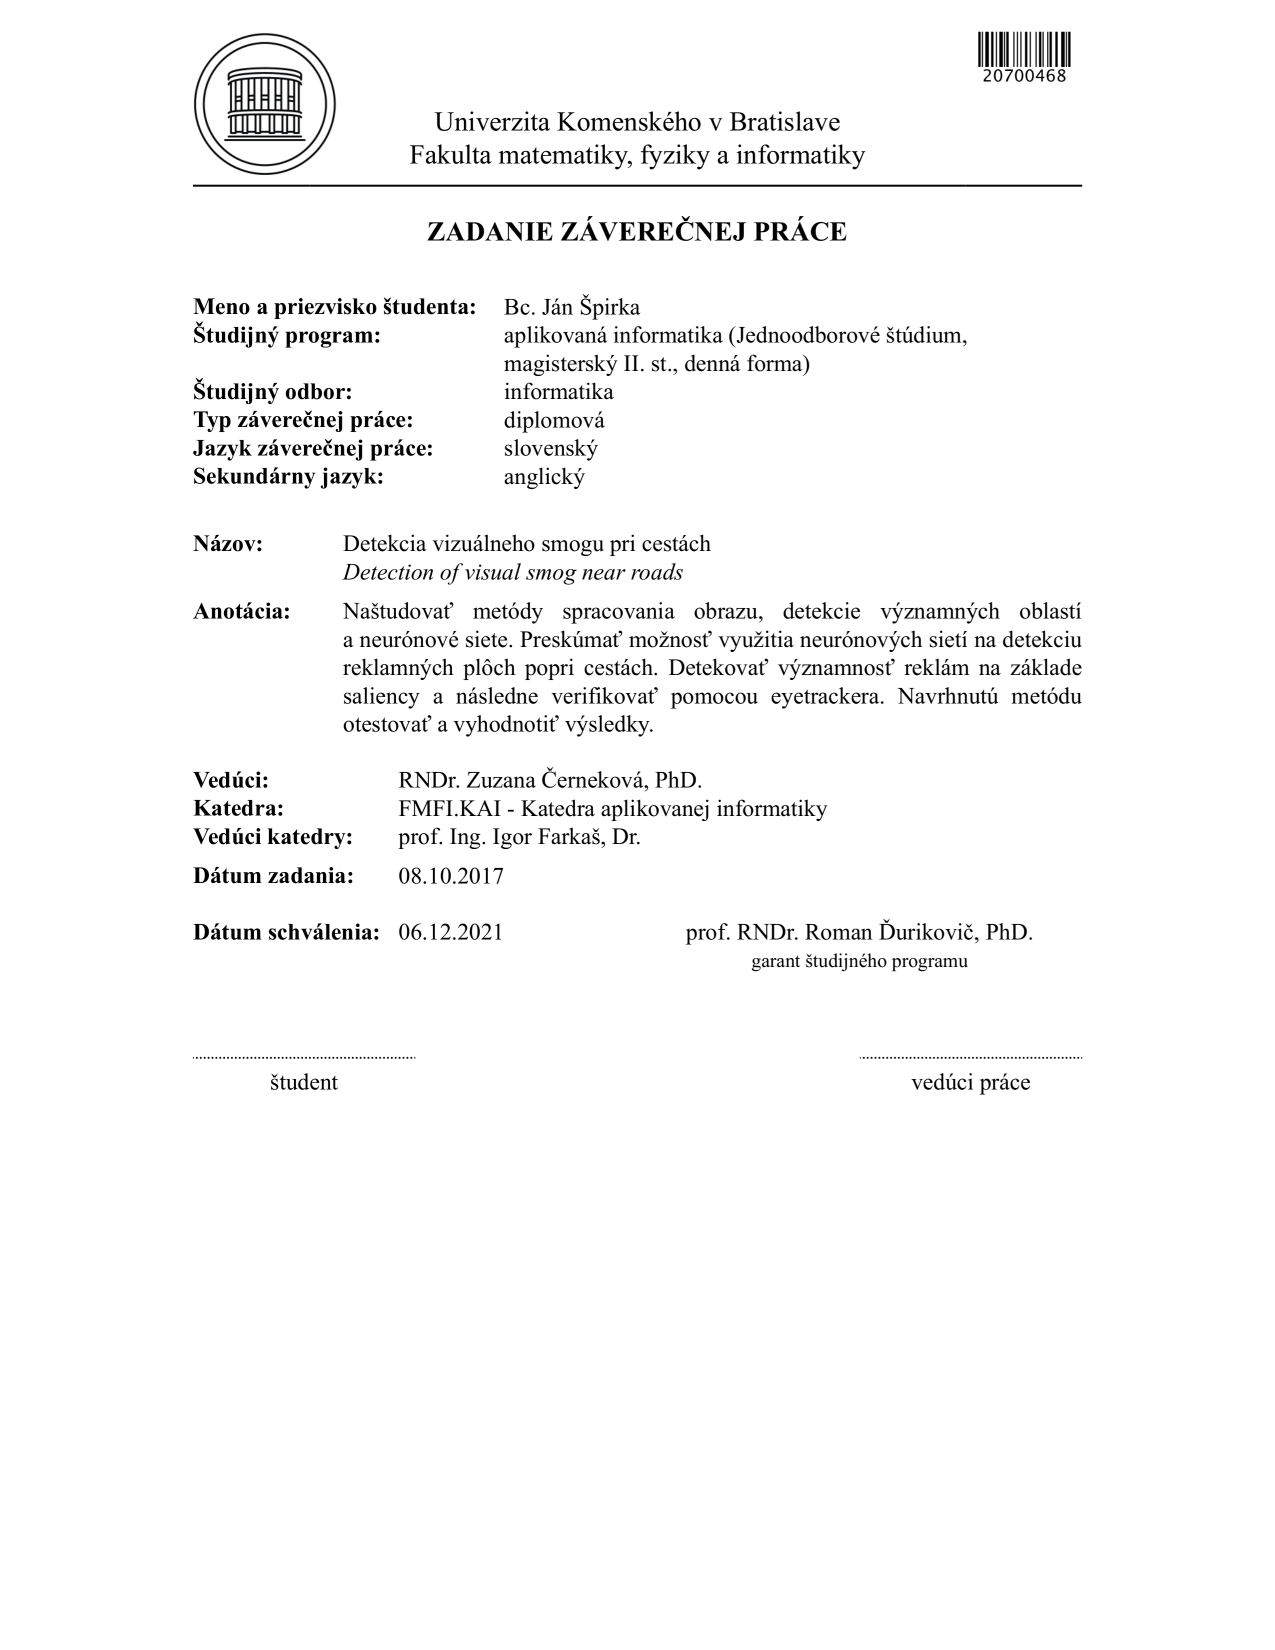
\includegraphics[width=\paperwidth]{images/zadanie-prace.jpg}}
\label{img:zadanie}
\end{center}
\end{figure}

% Anotácia
% Naštudovať metódy spracovania obrazu, detekcie významných oblastí a neurónové siete. Preskúmať možnosť využitia neurónových sietí na detekciu reklamných plôch popri cestách. Detekovať významnosť reklám na základe saliency a následne verifikovať pomocou eyetrackera. Navrhnutú metódu otestovať a vyhodnotiť výsledky.

{~}\vspace{12cm}



% --------------------------------------
%                   PREHLASENIE
% --------------------------------------
\noindent
\begin{minipage}{0.25\textwidth}~\end{minipage}
\begin{minipage}{0.75\textwidth}
Čestne prehlasujem, že diplomovú prácu som vypracoval samostatne s použitím uvedenej literatúry a za pomoci konzultácií s mojím školiteľom.
\newline \newline
\end{minipage}
\vfill
~ \hfill {\hbox to 6cm{\dotfill}} \\
\mfplacedate \hfill \mfauthor
\vfill\eject 



% --------------------------------------
%                   PODAKOVANIE
% --------------------------------------
\chapter*{Poďakovanie}\label{chap:thank_you}
Ďakujem školiteľke diplomovej práce, RNDr. Zuzane Černekovej, PhD, za pomoc a odborné vedenie, ktoré mi poskytla pri vypracovaní diplomovej práce. Všetkým účastníkom experimentu, priateľke a rodine za pomoc a podporu počas písania tejto práce.
\vfill\eject 


% --------------------------------------
%                   ABSTRAKT
% --------------------------------------


% veľmi krátke zhrnutie (jeden odsek, cca ¼ strany) výsledkov práce
% mal by byť pochopiteľný bežnému odborníkovi z vášho odboru, resp. vášmu spolužiakovi, aj keď sa nevenuje podobným témam
% zvykne sa zverejňovať aj samostatne, nepoužívajú sa preto skratky a označenia zavedené v práci
% uvádza sa aj 3-5 kľúčových slov

\chapter*{Abstrakt}\label{chap:abstract_sk}
Hlavným cieľom našej práce je preskúmať detekciu reklamných plôch popri cestách s využitím neurónových sietí. Následne takýmto reklamám určiť ich významnosť a to potom overiť pomocou eyetrackera.

Teoretická časť obsahuje dve časti. V prvej kapitole sa venujeme zadefinovaniu pojmov týkajúcich sa detekcie objektov a významnosti reklám. Na to nadviažeme v druhej kapitole, ktorá je teoreticky zameraná na neurónové siete a prácu s nimi. Ďalšie časti práce sa venujú praktickému riešeniu. Tretia kapitola obsahuje návrh nášho riešenia, ktoré v štvrtej kapitole realizujeme. Výstupy z našej práce sú zhrnuté v poslednej, piatej časti práce.

~\\
Kľúčové slová: neurónové siete, detekcia reklám, klasifikátor
\vfill\eject



% --------------------------------------
%                   ABSTRACT
% --------------------------------------
\chapter*{Abstract}\label{chap:abstract_en}
The main goal of our work is to investigate the detection of advertising areas along the roads using neural networks. Subsequently, determine the significance of such advertisements and then verify this using the eyetracker.

The theoretical part contains two parts. In the first chapter, we are devoted to defining concepts related to object detection and their significance. We will follow up on this in the second chapter, which is theoretically focused on neural networks and working with them. Other parts of the work are devoted to practical solutions. The third chapter contains the proposal of our solution, which we implement in the fourth chapter. The results of our work are summarized in the last, fifth part of the work.

~\\
Keywords: neural networks, advertisement detection, classifier
\vfill\eject 



% --------------------------------------
%                   OBSAH
% --------------------------------------
\newpage
\tableofcontents


% --------------------------------------
%                   ZOZNAMY
% --------------------------------------
% \newpage 
% \listoffigures
% \listoftables



% --------------------------------------
%                   KAPITOLY
% --------------------------------------
\mainmatter

\input 00intro.tex
\input 01overview.tex
\input 02theory.tex
\input 03proposal.tex
\input 04research.tex
\input 05results.tex
\input 06conclusion.tex


% --------------------------------------
%                   BIBLIOGRAFIA
% --------------------------------------
\backmatter

\nocite{*}
\bibliographystyle{unsrt}
\bibliography{references}

\end{document}